\documentclass{article}
\usepackage[utf8]{inputenc}
\usepackage{dsfont}
\usepackage{float}
\usepackage{amsmath}
\usepackage{graphicx}
\usepackage[colorinlistoftodos]{todonotes}
\usepackage[colorlinks=true, allcolors=blue]{hyperref}
\usepackage{algpseudocode}
\usepackage{algorithm}

\title{Métodos Constructivos}
\author{Camilo Andrés Rodríguez Garzón}

\author{Camilo Andrés Rodríguez Garzón}
\date{\today}

\begin{document}
\maketitle

\section{Descripción}
En el presente trabajo se desea resolver el problema del viajante. Para esto, se elaboró tres métodos aleatorios que permitiecen obtener una ruta y de esta manera resolver dicho problema. Para este trabajo se eligieron el método Búsqueda Aleatoria en la región factible, Estrategia Evolutiva (1+1) y Recocido Simulado (url con implementación de los métodos \href{https://github.com/camilorodriguezga/Tsp}{Tsp}
). A continuación se presenta el algoritmo correspondiente a cada uno de los métodos:

\begin{algorithm}[H]
	\caption{Random Search Tsp}\label{RandomSearchTsp}
	\begin{algorithmic}[1]
		\Procedure{Build Route}{N}
		\State $d, coorR \gets generateRandomSolution(coordinates)$ \Comment{obtener una solución inicial aleatoria y su distancia}
		\State $k \gets 1$ \Comment{inicializa número de iteraciones}
		\While{$k < N$}
		\State $dt, rs \gets generateRandomSolution(coordinates)$ \Comment{obtener una solución aleatoria y su distancia}
		\If {$dt<d$} \Comment{si la nueva solución es mejor}
		\State $d \gets dt$
		\State $coorR \gets rs$
		\EndIf
		\State $k \gets k+1$
		\EndWhile\label{euclidendwhile}
		\State $drawTsp(coorR, d)$ \Comment{se dibuja la solución obtenida}
		\EndProcedure
	\end{algorithmic}
\end{algorithm}

\begin{algorithm}[H]
	\caption{Evolutionary Strategy Tsp}\label{EvolutionaryStrategyTsp}
	\begin{algorithmic}[1]
		\Procedure{Build Route}{N}
		\State $newCoor \gets copy(coordinates)$\Comment{obtener una copia de las coordenadas}
		\State $dF, coorF \gets generateFather(coordinates)$ \Comment{obtener una solución inicial padre y su distancia}
		\State $k \gets 1$ \Comment{inicializa número de iteraciones}
		\While{$k < N$}
		\State $dS, coorS \gets generateMutation(dF, coorF)$ \Comment{obtener una solución hija y su distancia con una mutación dada}
		\If {$dt<d$} \Comment{si la nueva solución es mejor}
		\State $dF \gets dS$
		\State $coorF \gets coorS$
		\EndIf
		\State $k \gets k+1$
		\EndWhile\label{euclidendwhile}
		\State $drawTsp(coorR, d)$ \Comment{se dibuja la solución obtenida}
		\EndProcedure
	\end{algorithmic}
\end{algorithm}

\begin{algorithm}[H]
	\caption{Simulated Annealing Tsp}\label{SimulatedAnnealingTsp}
	\begin{algorithmic}[1]
		\Procedure{Build Route}{N}
		\State $tk \gets 100$\Comment{la temperatura se inicializa en 100}
		\State $alpha \gets 0.98$\Comment{la tasa de variación de la temperatura se inicializa en 0.98}
		\State $newCoor \gets copy(coordinates)$\Comment{obtener una copia de las coordenadas}
		\State $dF, coorF \gets generateFather(coordinates)$ \Comment{obtener una solución inicial padre y su distancia}
		\State $k \gets 1$ \Comment{inicializa número de iteraciones}
		\While{$k < N$}
		\State $dS, coorS \gets generateMutation(dF, coorF)$ \Comment{obtener una solución hija y su distancia con una mutación dada}
		\If {$dt<d$} \Comment{si la nueva solución es mejor}
		\State $dF \gets dS$
		\State $coorF \gets coorS$
		\Else
		\State $pa \gets e (- \left | dF-dS \right | / tk)$\Comment{probabilidad de aceptación}
		\State $tk \gets tk * alpha$\Comment{decrementar la temperatura}
		\State $ra \gets random(1, 0)$\Comment{random de aceptación}
		\If {$ra < pa$}\Comment{aceptar solución menos factible}
		\State $dF \gets dS$
		\State $coorF \gets coorS$
		\EndIf
		\EndIf
		\State $k \gets k+1$
		\EndWhile\label{euclidendwhile}
		\State $drawTsp(coorR, d)$ \Comment{se dibuja la solución obtenida}
		\EndProcedure
	\end{algorithmic}
\end{algorithm}

Es de resaltar que para obtener una solución hija se realizo swaping entre dos coordenadas, una coordenada inicial aleatoria del padre y una coordenada cercana a la coordenada inicial y así posteriormente obtener una solución hija recalculando la distancia total.

En relación a la temperatura y a decremente de este (alpha) se realizaron varias muestras que permitieron ver mejores comportamientos con dichos valores iniciales.

La solución inicial se obtiene atra vez de la construcción del Tsp usando como algoritmo base nearest neighbors y esta cota primar se toma como pie de apoyo para la obtención de nuevas soluciones.

Se eligió dichos métodos y esto se resume al hecho de aprender en un ambiente más real cuales son las dificultades de implementarlos así como también de adquirir la experiencia de poder construir cada unos de estos.

\section{Resultados}

\subsection{Datos linhp318}

\begin{figure}[H]
	\begin{minipage}{0.33\textwidth}
		\centering
		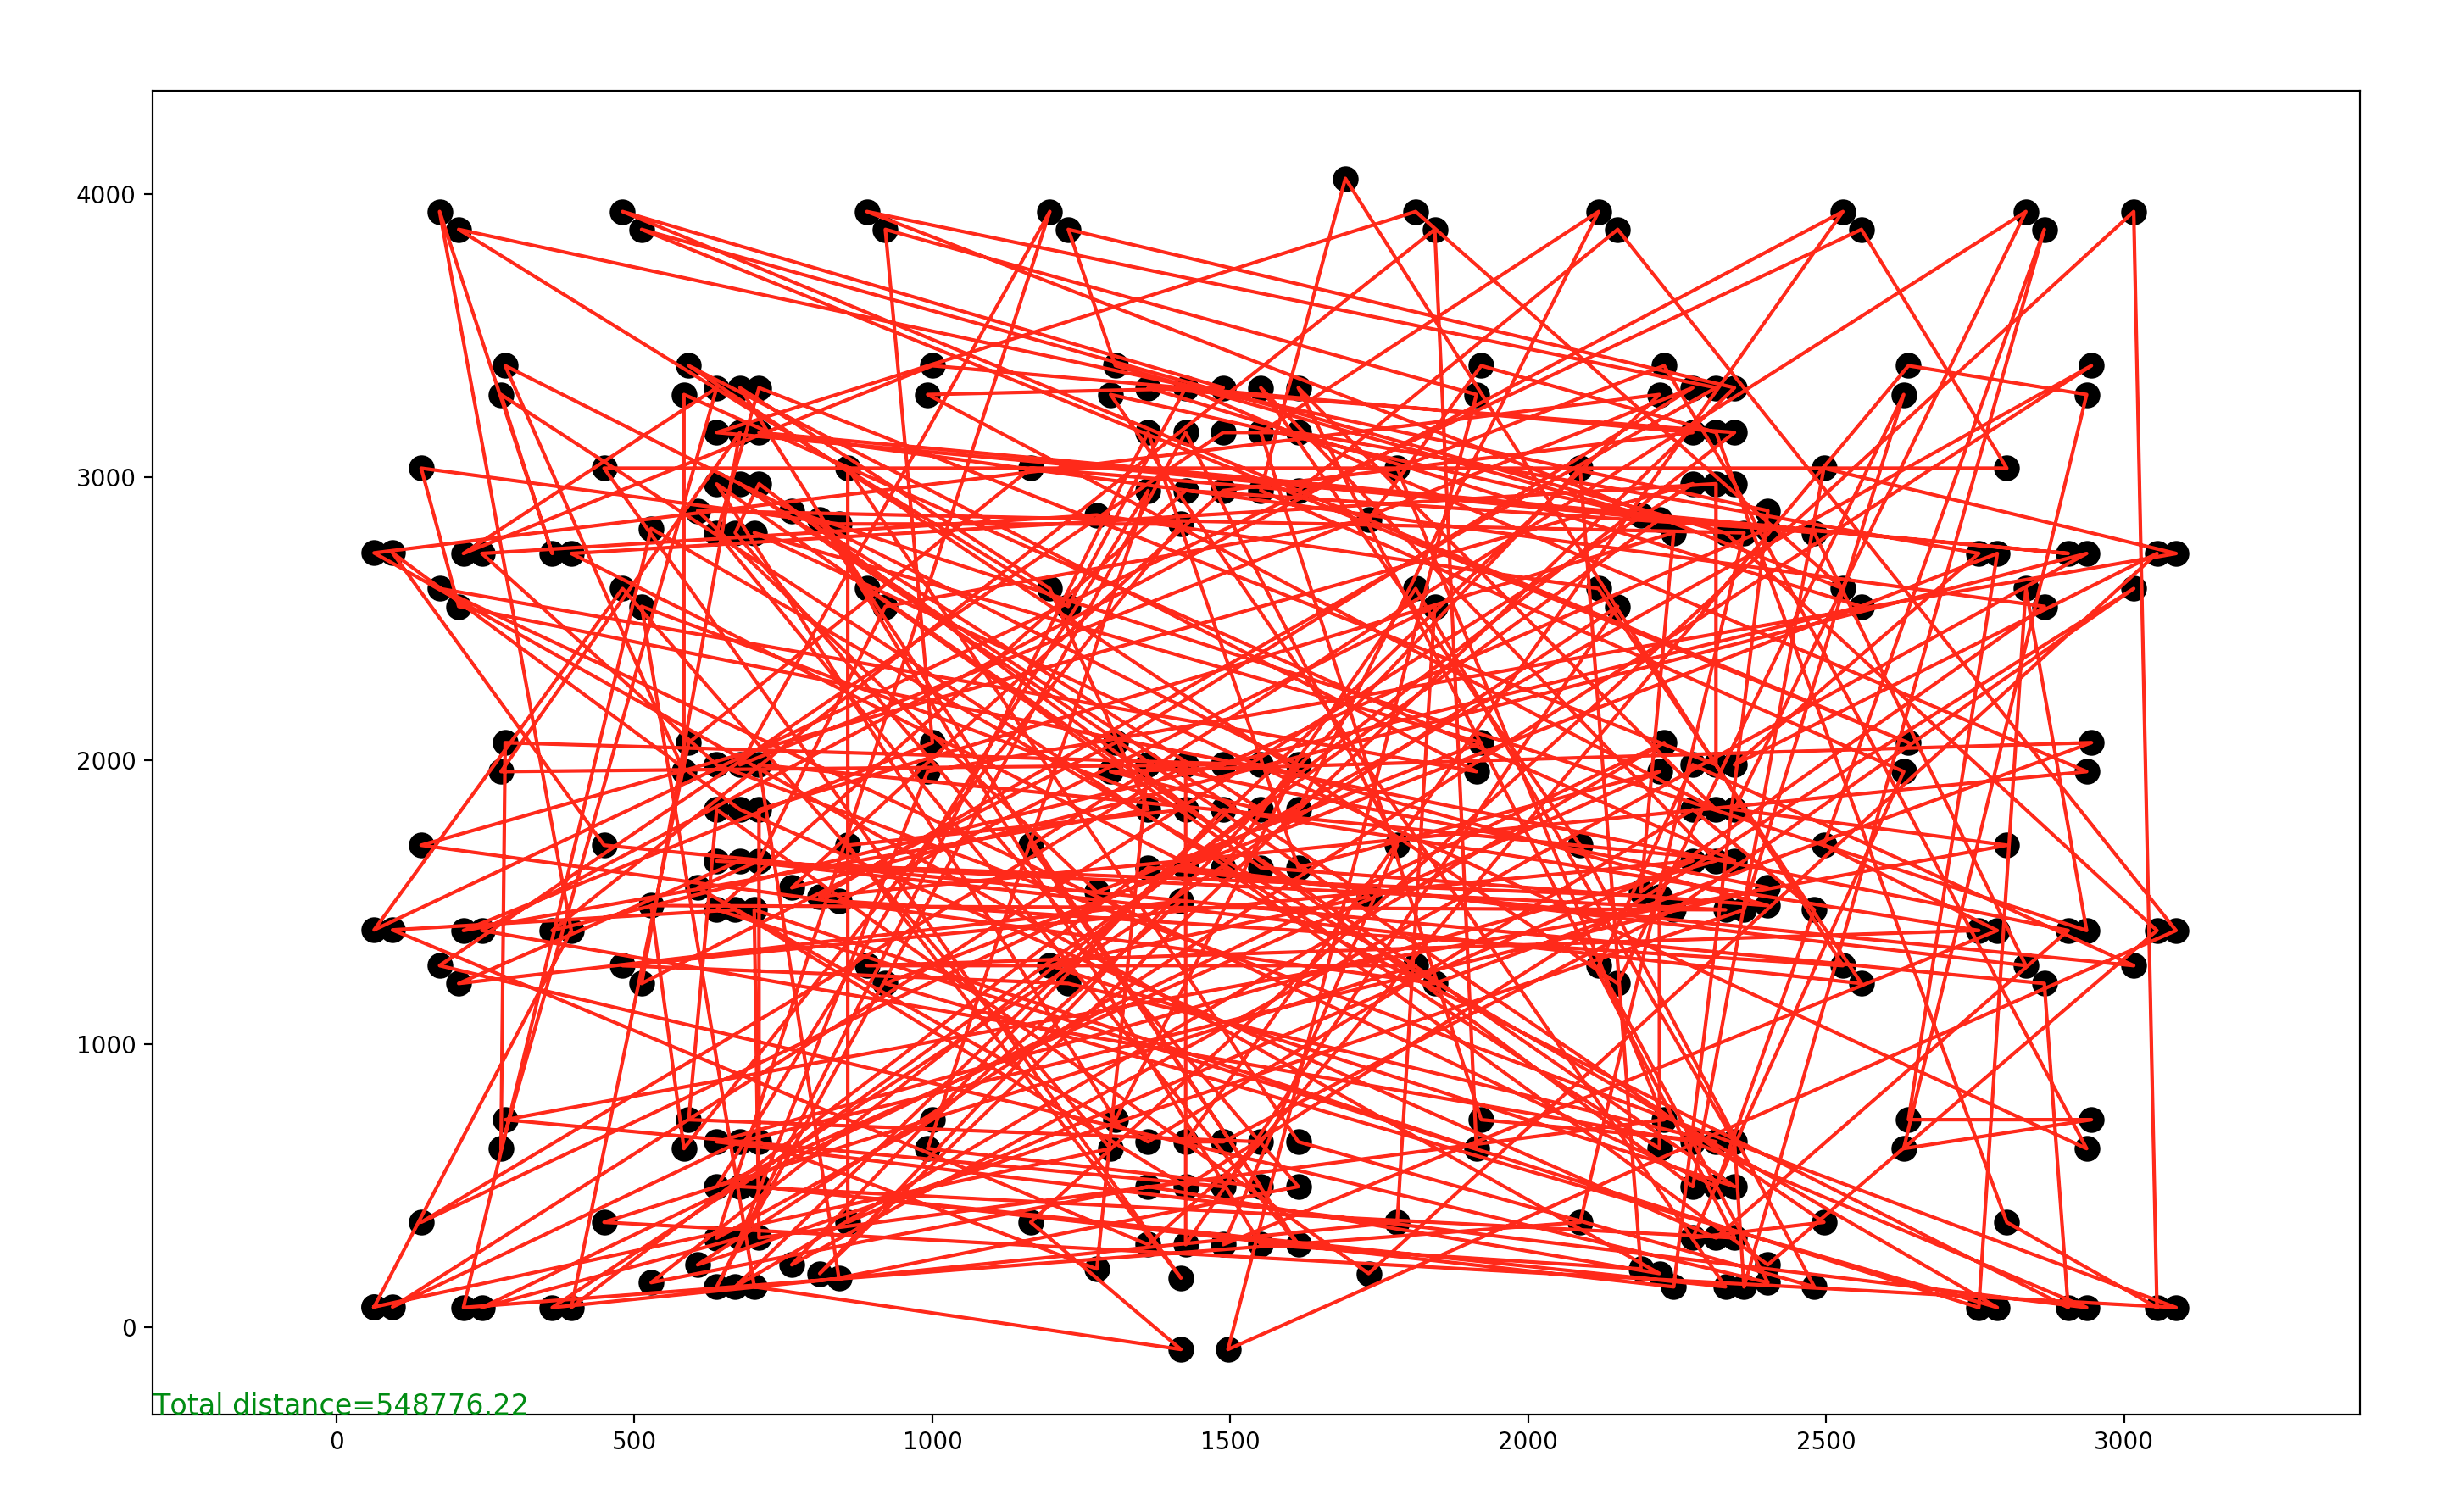
\includegraphics[width=1\textwidth]{../../image/randomsearch/linhp318.png}
		\caption{\label{fig:Figura1} Tsp random search}
	\end{minipage}\hfill
	\begin {minipage}{0.33\textwidth}
		\centering
		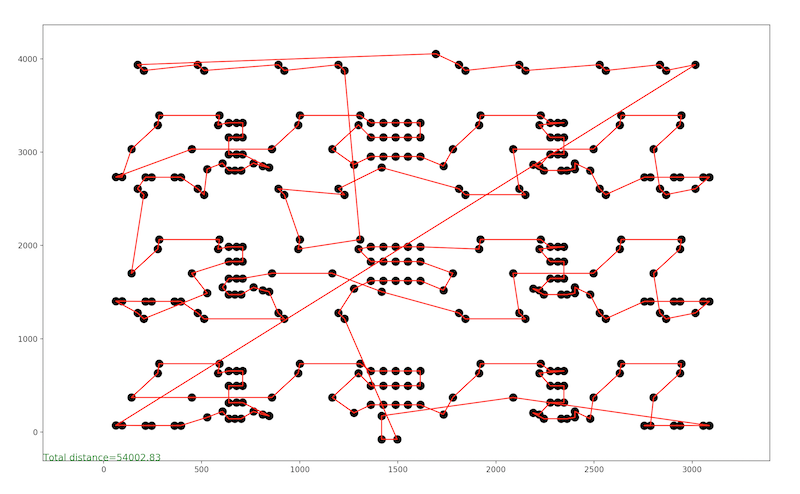
\includegraphics[width=1\textwidth]{../../image/evolutionarystrategy/linhp318.png}
		\caption{\label{fig:Figura1} Tsp evolutionary strategy}
	\end{minipage}
	\begin {minipage}{0.33\textwidth}
	\centering
	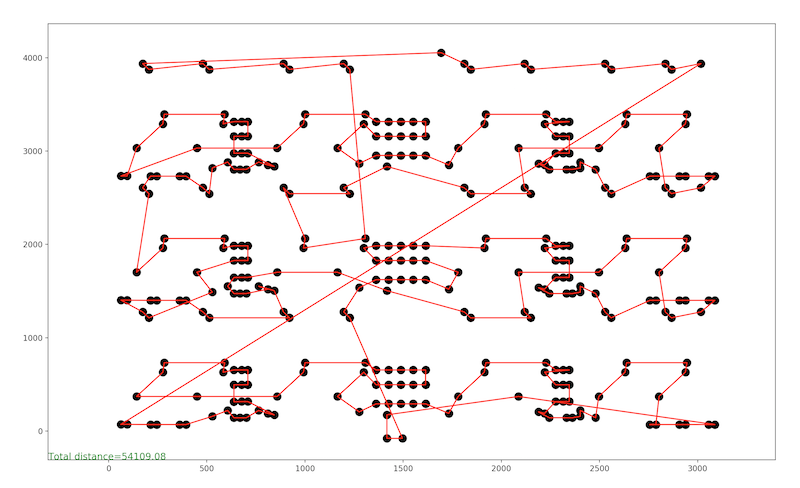
\includegraphics[width=1\textwidth]{../../image/simulatedannealing/linhp318.png}
	\caption{\label{fig:Figura1} Tsp simulated annealing}
	\end{minipage}
\end{figure}

\begin{table}[H]
\centering
\caption{Comparativa de tiempo de ejecución y distancia recorrida de Algoritmos para linhp318}
\label{Table:linhp318}
\begin{tabular}{| l | l | l | l |}
\hline
Algoritmo & Tiempo Inicial & Tiempo final & Distancia \\ \hline
Random search & 2018-03-20 01:42:36.915734 & 2018-03-20 01:42:37.509704 & 548776.22 \\ \hline
Evolutionary strategy & 2018-03-20 01:38:42.038569 & 2018-03-20 01:38:45.149977 & 54002.83 \\ \hline
Semi-pilot & 2018-03-20 01:44:23.633350 & 2018-03-20 01:44:26.755945 & 54109.08 \\ \hline
TSPLIB & - & - & 41345 \\ \hline

\end{tabular}
\end{table}

\subsection{Datos berlin52}

\begin{figure}[H]
	\begin{minipage}{0.33\textwidth}
		\centering
		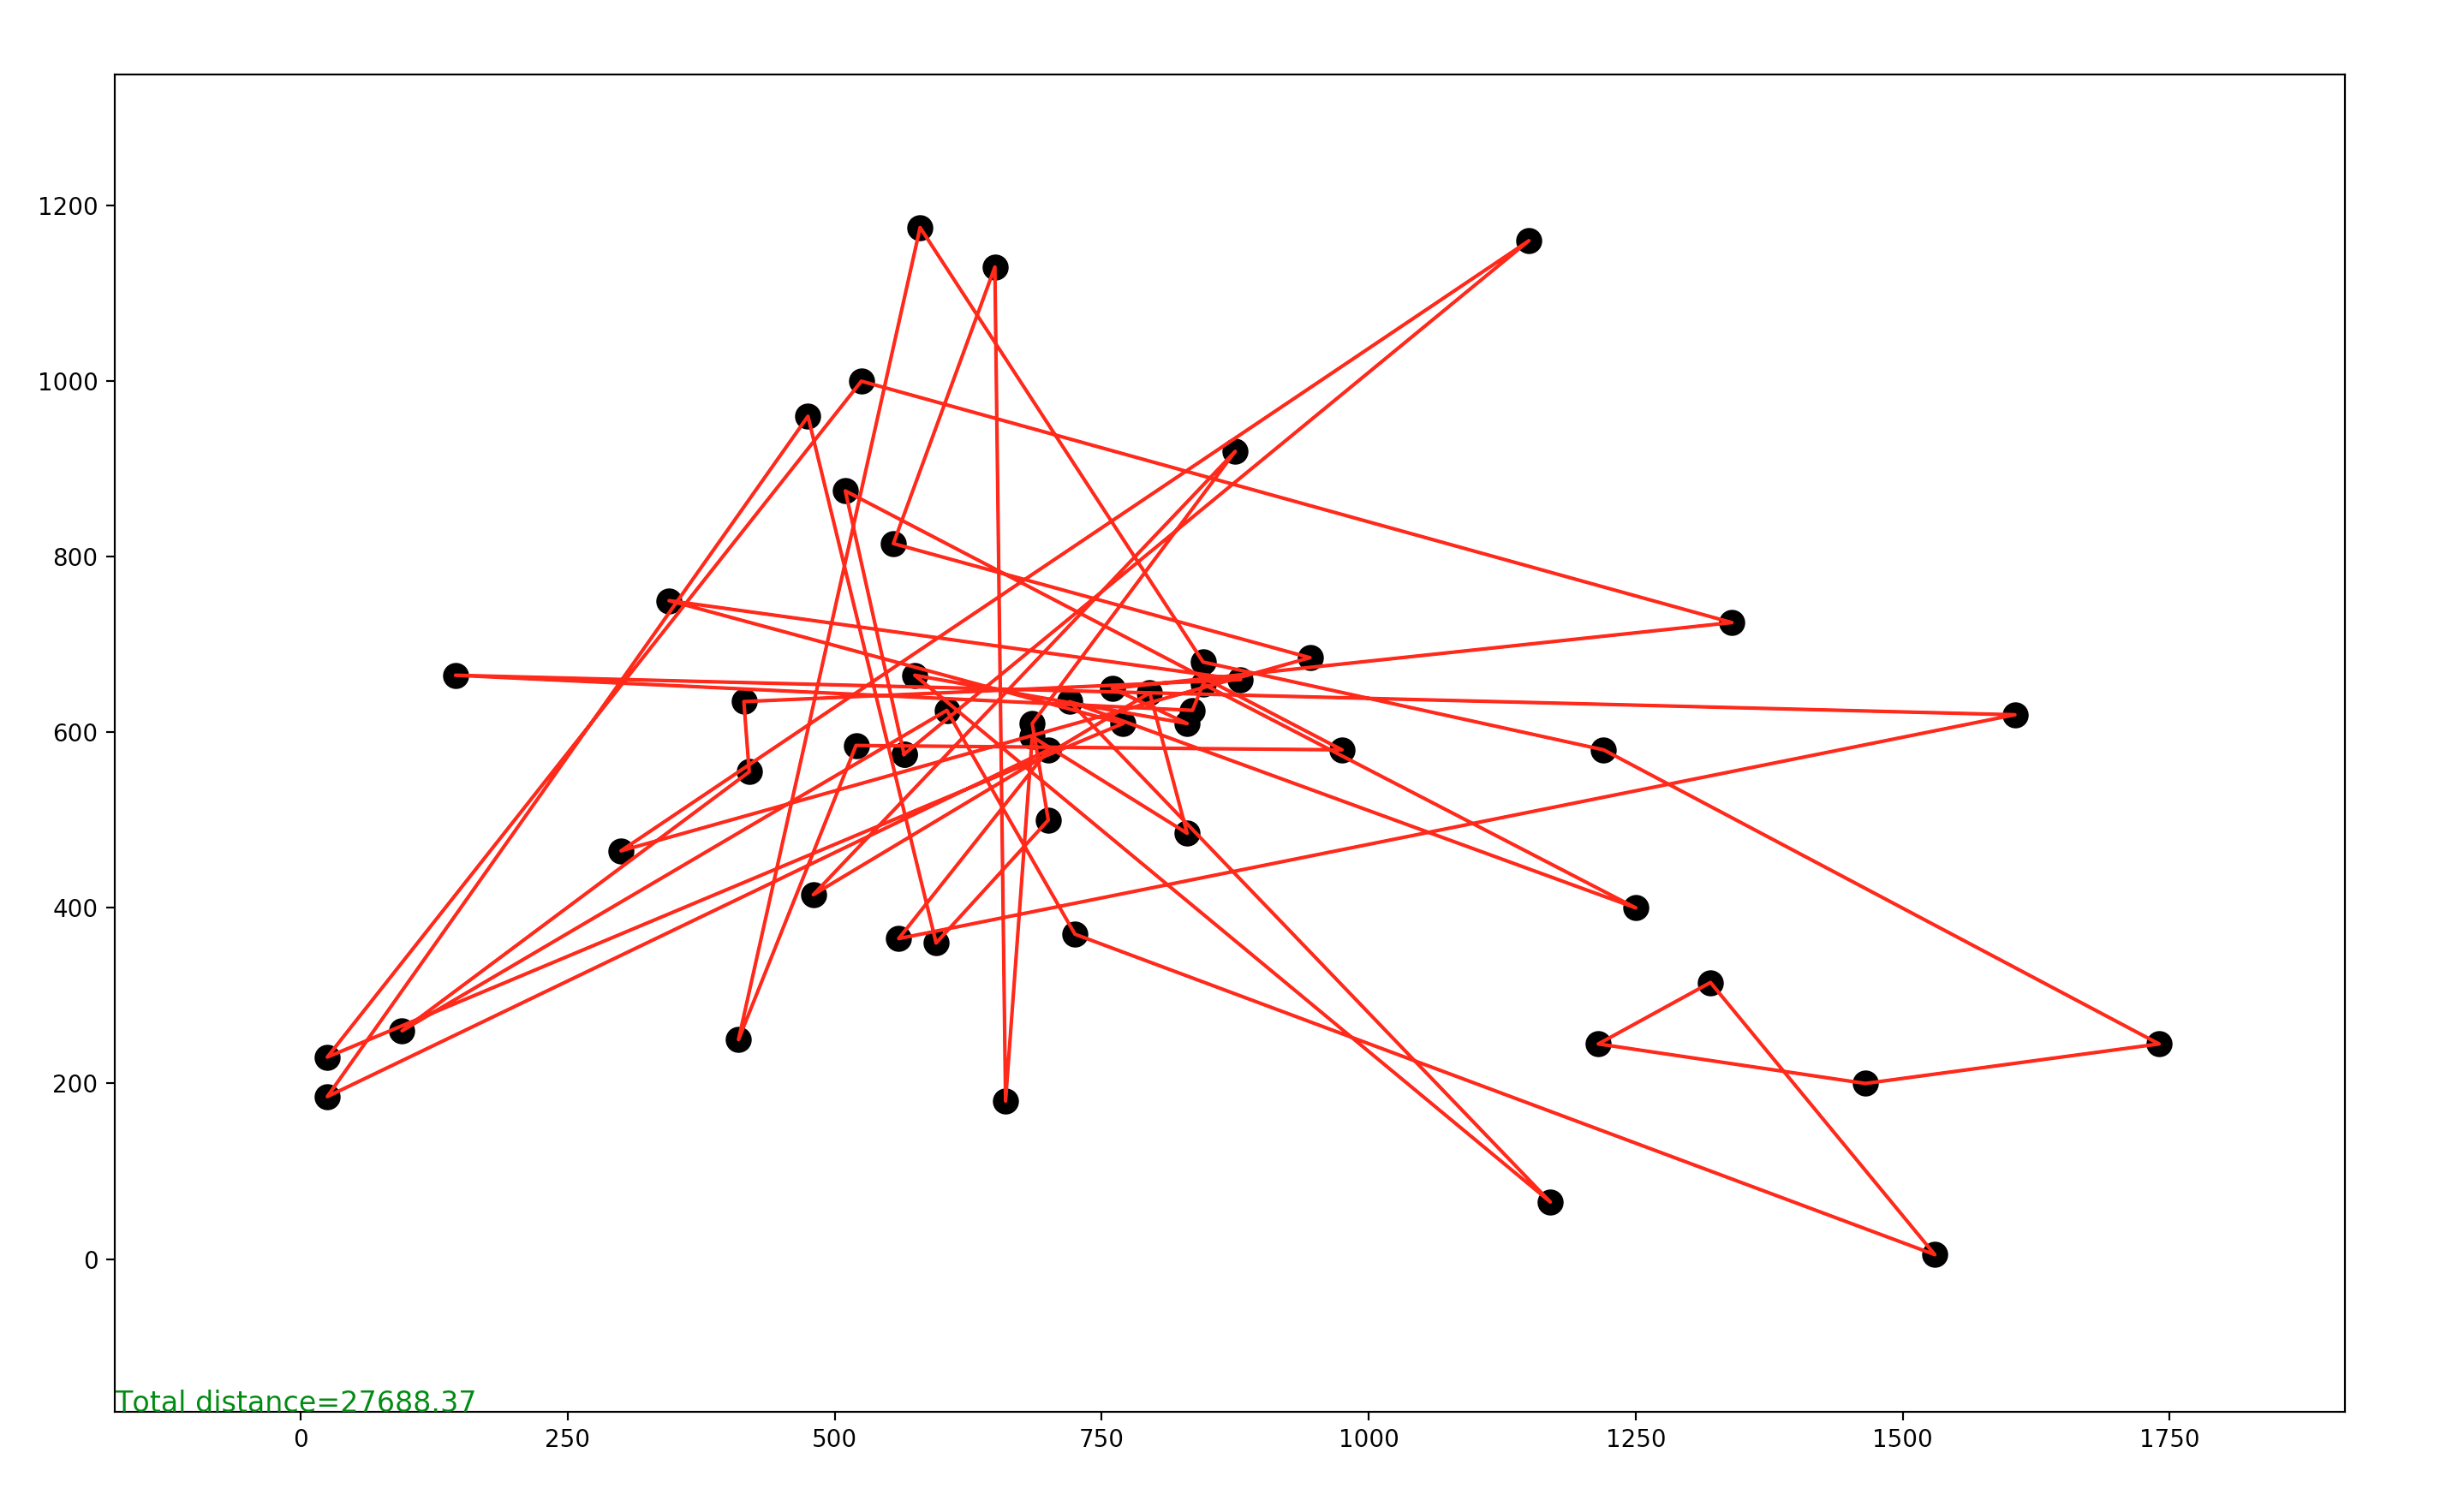
\includegraphics[width=1\textwidth]{../../image/randomsearch/randomsearch-berlin52.png}
		\caption{\label{fig:Figura1} Tsp random search}
	\end{minipage}\hfill
	\begin {minipage}{0.33\textwidth}
	\centering
	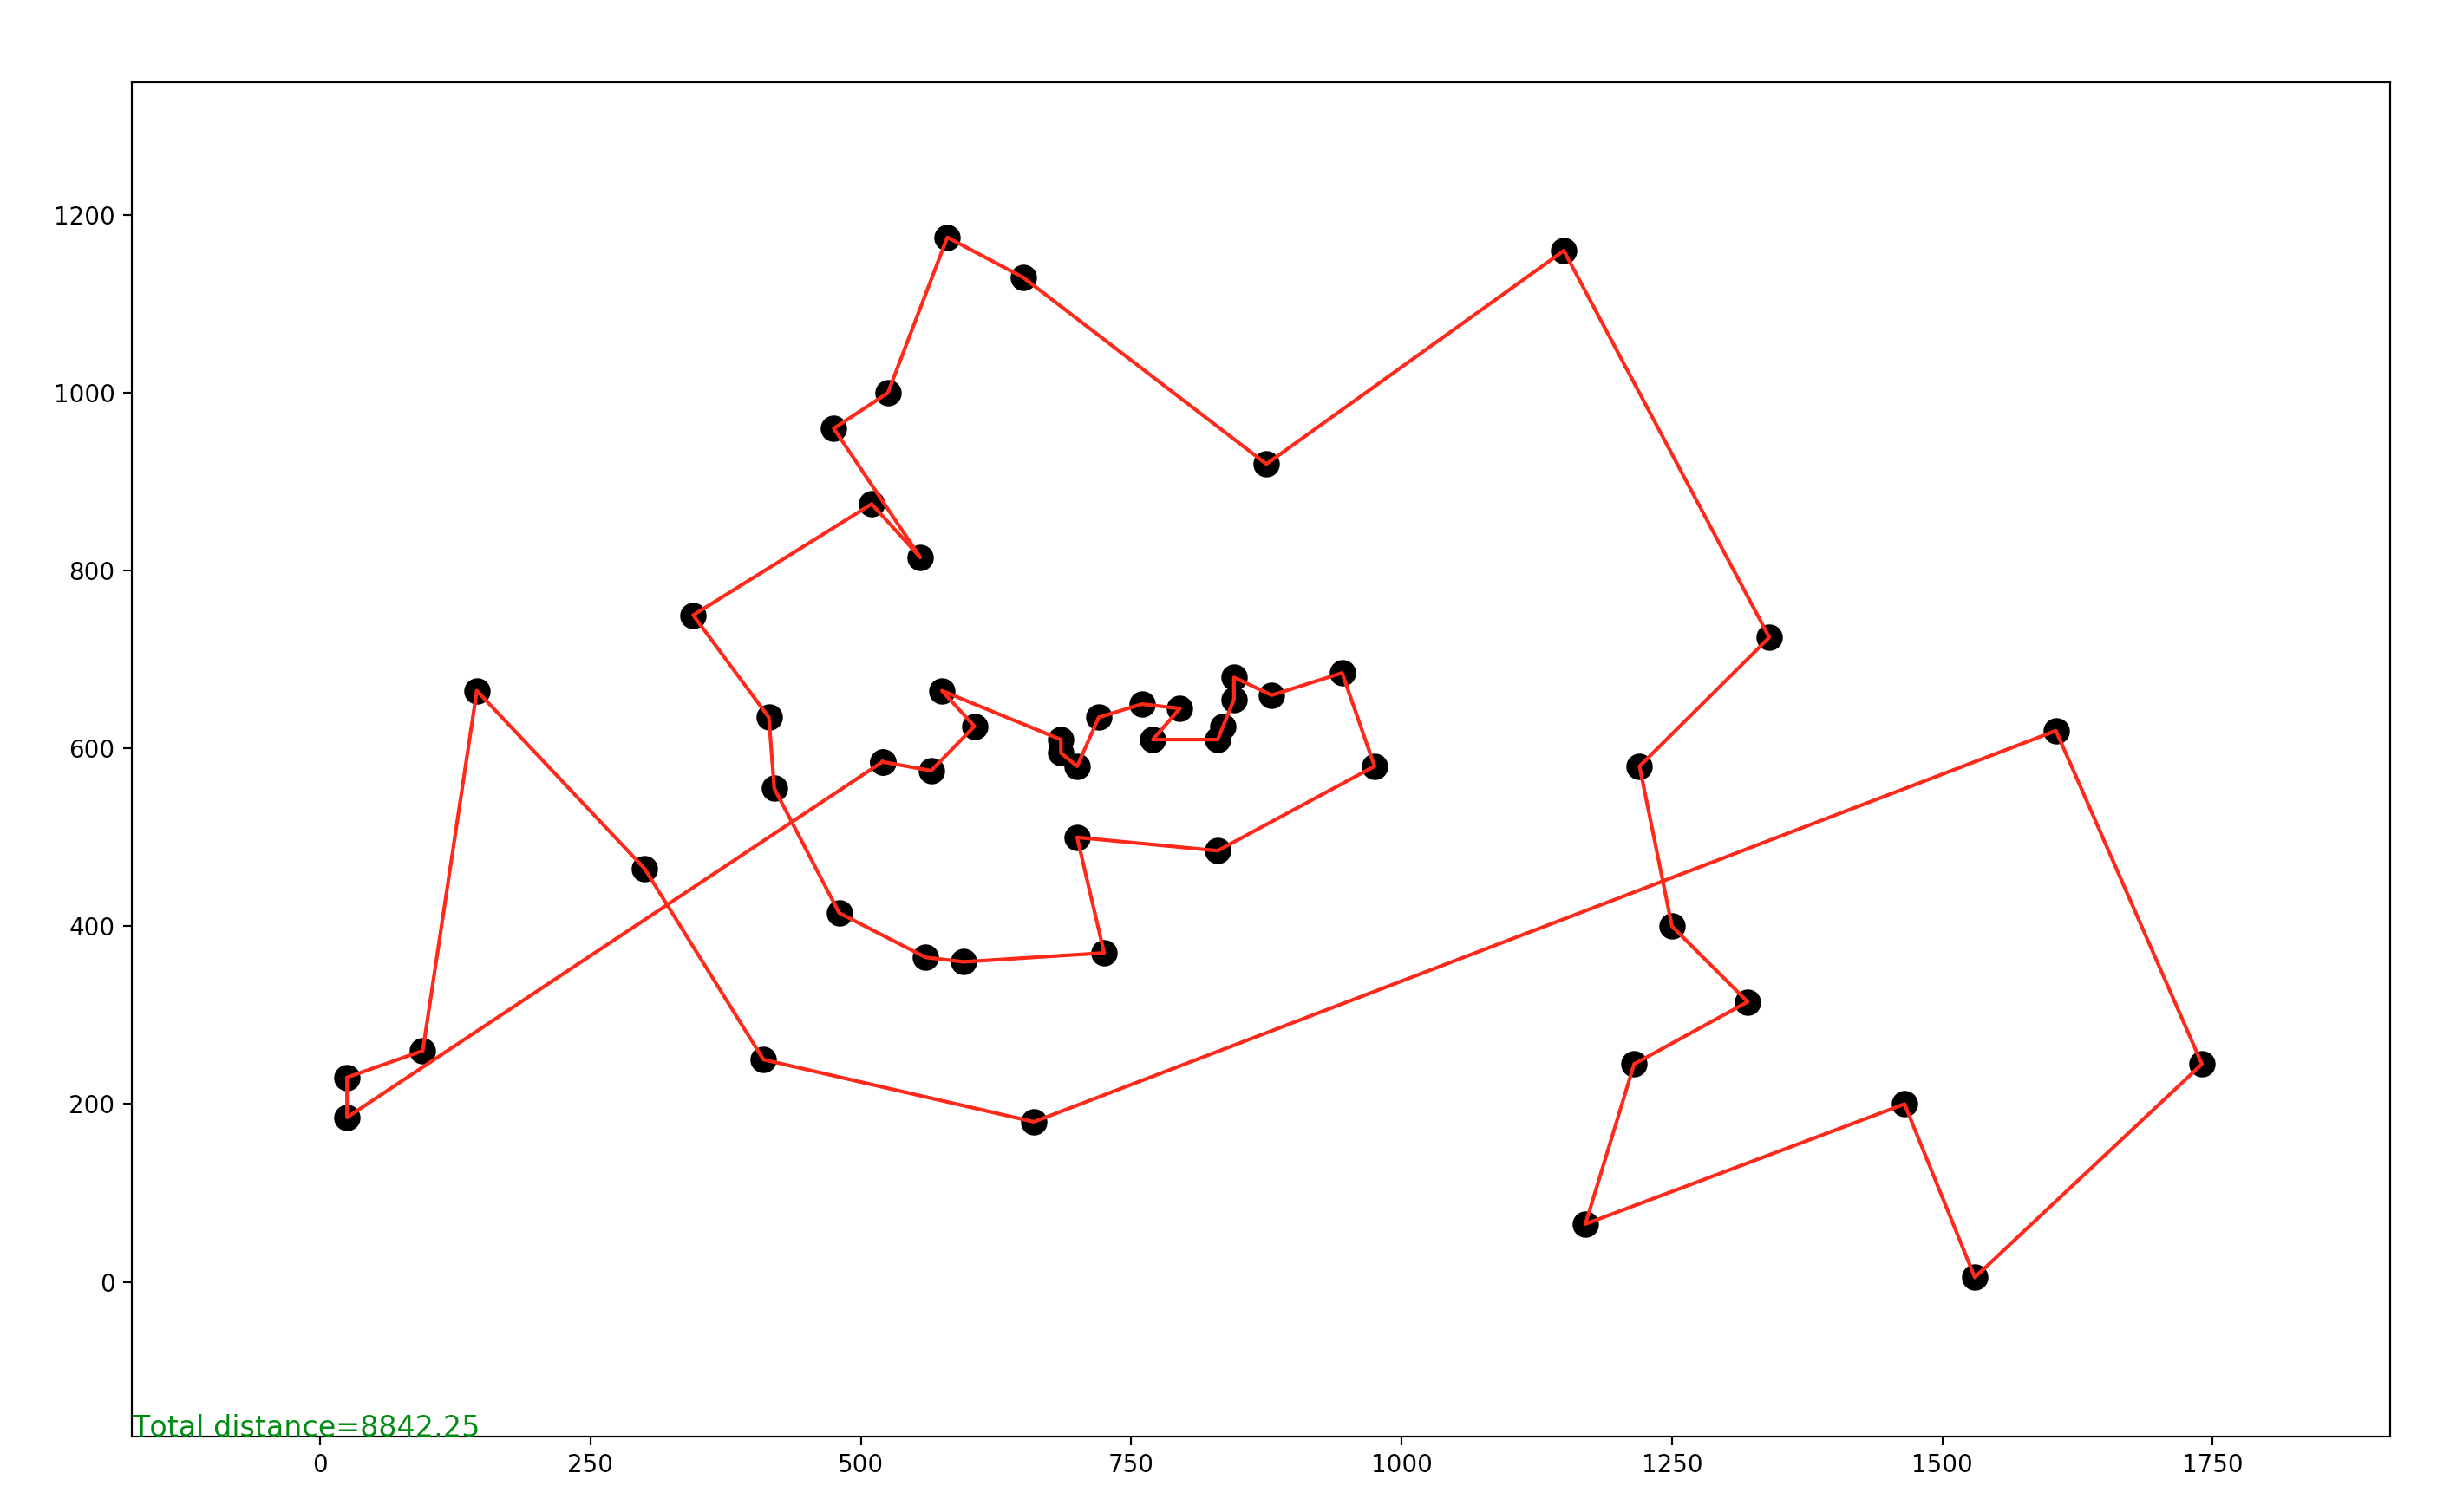
\includegraphics[width=1\textwidth]{../../image/evolutionarystrategy/evolutionarystrategy-berlin52.png}
	\caption{\label{fig:Figura1} Tsp evolutionary strategy}
\end{minipage}
\begin {minipage}{0.33\textwidth}
\centering
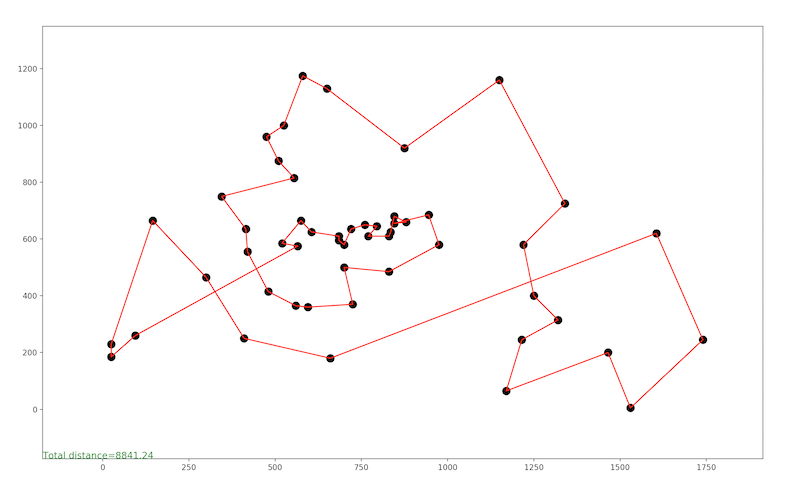
\includegraphics[width=1\textwidth]{../../image/simulatedannealing/simulatedannealing-berlin52.png}
\caption{\label{fig:Figura1} Tsp simulated annealing}
\end{minipage}
\end{figure}

\begin{table}[H]
\centering
\caption{Comparativa de tiempo de ejecución y distancia recorrida de Algoritmos para berlin52}
\label{Table:berlin52}
\begin{tabular}{| l | l | l | l |}
\hline
Algoritmo & Tiempo Inicial & Tiempo final & Distancia \\ \hline
Random search & 2018-03-20 01:33:02.365071 & 2018-03-20 01:33:02.702718 & 27688.37 \\ \hline
Evolutionary strategy & 2018-03-20 01:33:50.417394 & 2018-03-20 01:33:52.613921 & 8976.29 \\ \hline
Simulated annealing & 2018-03-20 01:34:58.561924 & 2018-03-20 01:35:00.775077 & 8932.06 \\ \hline
TSPLIB & - & - & 7542 \\ \hline

\end{tabular}
\end{table}

\section{Conclusiones}
\begin{itemize}
\item El algoritmo de simulado recodido arrojó mejor solución en los datos de berlin52 pero en los datos de linhp318 lo hizo la estrategía evolutiva, lo que nos hace pensar que siempre hay que calibrar la temperatura y el decremento de está para que el simulado recocido se comporte de una mejor manera.
\item Los tiempos de ejecución son más extensos en el algoritmo de simulado recocido y la estrategia evolutiva, esto es debido a la evaluación de el camino padre e hijo.
\item El método del vecino más cercano es un algoritmo muy potente en relación a los tiempos de ejecución y tomando este como cota primal se hace muy dificil mejorar la solución ya obtenida.
\item Ambos algoritmos por la estrategia greedy que manejan son castigados al unir la coordenada final con la inicial.
\item Las implementaciones realizadas en TSPLIB superan significativamente a las soluciones construidas.
\end{itemize}

\end{document}
